% Chapter 1
%\begin{multicols}{2}

\section{Introduction to Wireless Sensor Networks} % Main chapter title
\label{Section1} % To reference to this chapter elsewhere, use \ref{Section1} 
%\lhead{Chapter 1. \emph{Sound nomenclature}} % This is for the header on each page - perhaps a shortened title
%\textsf{\textsl{Written by Bjorn Deraeve}}
%----------------------------------------------------------------------------------------
%\begin{center}
%{\textsl{What if: }}
%\begin{large}
%\textbf{Ubiquitous Computing \& Networking} + \textbf{Sensing \& Control} ?
%\end{large}
%\end{center}
\subsection{Introduction}
The ENIAC\footnote{Electronic Numerical Integrator And Computer (ENIAC)}, the first electronic computer designed by American scientists J. Presper Eckert and John W. Mauchly, Turing-complete,  pioneering in 1946 and designed to calculate artillery firing tables \citep{FLAMM}. A wireless sensor network node, over 50 years later, 10 million times smaller than the ENIAC, still Turing-complete, and still military roots. The origins of the research in Wireless Sensor Networks (WSNs) can be traced back to DARPA\footnote{Defense Advanced Research Projects Agency (DARPA), is an American agency responsible for developing military technologies. DARPA has fund the research in many technologies which have had major effect on the world, including ARPANET, the first wide-area packet switching network (ancestor of the Internet) and Douglas Engelbart's precursors to the graphical user interface (GUI)\citep{DARWIKI}.},which sponsored a workshop at Carnegie Mellon University\begin{wrapfigure}[9]{r}[\dimexpr.5\width+.5\columnsep\relax]{4cm}
  \centering
  \parbox{4cm}{\textsl{What if: }
\begin{large}
\textbf{\\Ubiquitous Computing \& Networking} \begin{center}+\end{center} \textbf{Sensing \& Control} ?
\end{large}}
  %\rule{5cm}{2.5cm}
\end{wrapfigure} in 1978, identifying the technology components for a Distributed Sensor Network (DSN) \citep{DAR}. But at the time the technology was not quite ready. Sensors could take up the size of a shoe box and up, limiting the number of potential applications. The earliest DSNs were also not very tightly associated with wireless communication. In 1998 a new wave of research in WSNs started. Again DARPA acted as a pioneer by launching the initiative research program 'SensIT', which added new capabilities to the current sensor networks such as ad hoc networking, dynamic querying and tasking, reprogramming and multi-tasking. At the same time the IEEE\footnote{Institute of Electrical and Electronics Engineers (IEEE)} noticed the high capabilities and low expenses of WSNs and defined the IEEE 802.15.4 standard for low power consumption, low data rate wireless PANs\footnote{Personal Area Network (PAN)} for 868MHz, 915MHz and 2.4GHz radios. Finally, in 2002, the ZigBee Alliance was established and published the ZigBee standard, based on IEEE 802.15.4. The standard adds a suite of high level communication protocols for WSNs such as device coordination, network topologies and interoperability with other wireless products.\\
Currently, WSNs are seen as one of the most prospective technologies of the 21st century \defcitealias{BW}{21 ideas for the 21st century, 1999}\citepalias{BW}. China for example, has involved WSNs in their national strategic research programs (Program 973)\citep{CHINA}. That project follows an application-driven methodology and aims to issues identified with the real-world critical problems facing Chinese society. Over the years the program has funded areas such as agriculture, health, resources, energy, population and materials and brought significant benefits to China's sustainable economic and social development.
%----------------------------------------------------------------------------------------
\subsection{Wireless is everywhere}
\subsubsection{Definition of Wireless Sensor Network}
\emph{A Wireless Sensor Network (WSN) consists of spatially distributed autonomous sensors connected via a (wireless) communications infrastructure to cooperatively monitor, record and store physical or
environmental conditions, such as temperature, sound, vibration, pressure, motion or pollutants} \citep{SEBA}
%---------------------------------
\subsubsection{Internet of Things}
The Internet of Things (IoT) is a term that was first used by Kevin Ashton\footnote{Kevin Ashton co-founded the Auto-ID Center at the  Massachusetts Institute of Technology (MIT). The Center is a research group in networked RFID and newly emerging sensing technologies. The main goal was the development of the Electronic Product Code (EPC), a global RFID-based item identification system intended to replace the UPC bar code \citep{AUTO}} in 1999 and answers the question introducing this chapter. It refers to uniquely identifiable objects (things) \begin{wrapfigure}[9]{l}[\dimexpr.5\width+.5\columnsep\relax]{3.5cm}
\vfill
\end{wrapfigure} and their virtual representation in an Internet-like structure. It is a vision of a network of Internet-enabled objects, combined with web services which interact with these objects. If all objects in the world would be equipped with minuscule identifying devices this could transform our daily lives. By embedding computational capabilities in all kinds of objects, including living beings, it will be possible to provide a qualitative and quantitative shift in several sectors: logistics, domotics, healthcare, entertainment, and so on.\\
WSNs provide a virtual layer where the information about the physical world can be accessed by any computational system. As a result, WSNs are one of the most important elements for realizing the vision of the Internet of Things paradigm \citep{ALCA}. On May 2nd, 2012, Libelium\footnote{The manufacturer of the Hardware we used. See chapter \ref{Chapter3} for more information.} published a list of 50 cutting edge \emph{Internet of Things} applications. According to Libelium, by 2020, more then 50 billion devices will be connected to the Internet \citep{50}.\\
The IoT can also be considered as the third wireless wave, following cellular technology and WiFi. Today wireless technology also includes the world of sense and control technology bridging the gap between the virtual electronic world and the human physical world \citep{ATLANTIC}.
%---------------------------------------------------------------------------------------- 
\subsection{Characteristics of a WSN}
\subsubsection{Node architecture}
A typical sensor node (mote) has the following components:
\begin{itemize}
\item Microcontroller (+ memory)
\item Transceiver
\item Sensors (+ ADCs)
\item Power supply
\end{itemize}
The main controller options are Microcontrollers, DSPs\footnote{Digital Signal Processor (DSP)}, FPGAs\footnote{Field-Programmable Gate Array (FPGA)} or ASICs\footnote{Application-Specific Integrated Circuit (ASIC)}. A microcontroller is the best option for a WSN node. They are general purpose and are optimized for embedded applications, so they use little power. DSPs are optimized for signal processing tasks and not suitable for WSNs. FPGAs can be good for testing purposes and ASICs are good if peak performance is needed without flexibility. The Libelium Waspmotes used for the test-bed have an 8-bit Atmel controller (see \ref{memory}).
%---------------------------------
\subsubsection{Fundamental Challenges in WSNs}
The biggest challenge WSNs encounter is without a doubt power consumption. Power! Power! Power! The next section will briefly introduce the general concepts and in section \ref{pow} the power consumption of the WSN we developed will be analyzed thoroughly. Other challenges often fall back to this limited amount of available energy, such as for example security.\\
There are dozens of other basic challenges for WSNs. Unattended operation and environmental influence makes a mote prone to failure. Mobility can cause topology changes. WSNs can use more than 100 nodes, this leads to scalability and synchronization issues. There must also be a form of synchronization with sleeping nodes, network responsiveness and robustness, not to forget making sense out of sensors.
%---------------------------------
\subsubsection{Power considerations}
\begin{figure}[t]%[htbp]
\centering
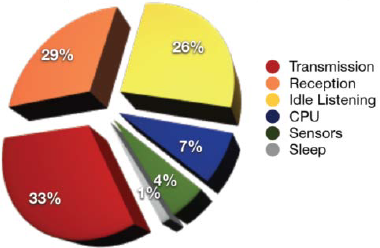
\includegraphics[width=0.3\textwidth]{typicalCons}
%\rule{30em}{0.5pt}
%\caption{Typical power consumption of a node}
%\label{fig:typicalCons}
\end{figure} 
%\vspace{1cm}
\begin{figure}[t]%[htbp]
\centering
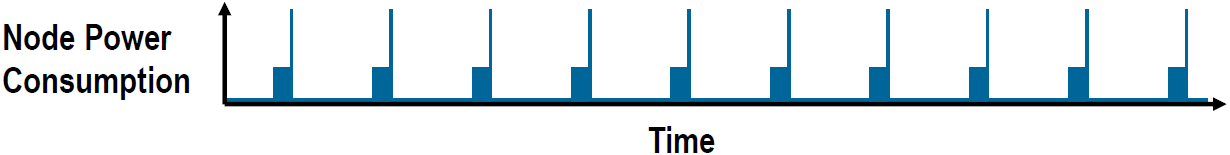
\includegraphics[width=0.48\textwidth]{powerCons}
%\rule{30em}{0.5pt}
\caption{The typical power consumption of a node}
\label{fig:typicalCons2}
\end{figure}
\noindent Figure \ref{fig:typicalCons2} shows a typical power usage division in a WSN node \citep{NIWSN}. Clearly the main power cost is due to Transmission / Networking. As a result, to obtain an acceptable battery life nodes must sleep most of the time. Effective use of network transmission (section \ref{powerSaver} ), effective dynamic power management (section \ref{dynPow}) and optimal duty cycles (section \ref{duty}) are the key to conserving power.\\
%---------------------------
\subsubsection{Benefits of Wireless Measurements}
Wireless Sensor Networks provide benefits in roughly three categories: installation and maintenance costs can be reduced, measurements can be optimized thus increasing efficiency, and finally infrastructure limitations can be overcome.
%-------------------------------------------------------------------
\subsection{Wireless Standards and Technology}
\subsubsection{Standards enable growth: ZigBee}
Not only do standards allow devices from different vendors to interoperate, they also provide OEMs\footnote{Original Equipment Manufacturer (OEM)} and integrators the flexibility of second sourcing. The ZigBee Alliance is an independent standardization organization which is driven by a large group of OEM companies and has definitely had a large impact on the rapid development of WSNs. Figure \ref{fig:stand} indicates the most critical properties of the ZigBee standard. Some rules-of-thumb are:
\begin{itemize}
\item The higher the frequency, the higher the data rate
\item The lower the frequency, the further the reach
\item All radio waves show strong absorption in water and metal 
\end{itemize}
\begin{figure}[t]%[htbp]
\centering
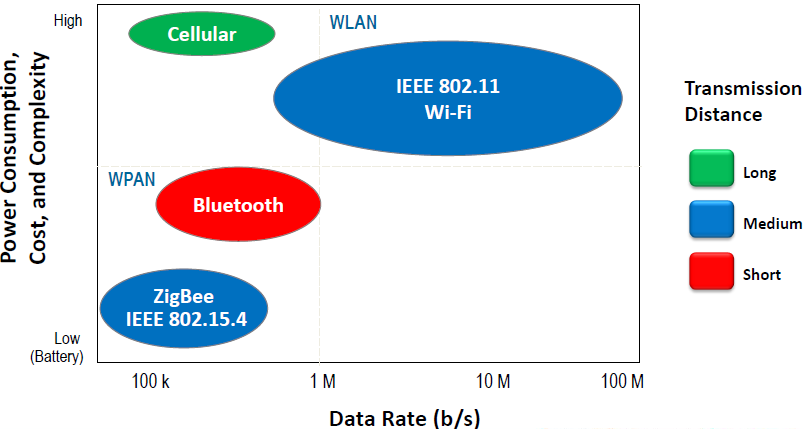
\includegraphics[width=0.48\textwidth]{zigbeeRange}
\caption{Comparing the ZigBee standard with Cellular, Bluetooth and WiFi}
\label{fig:stand}
\end{figure}
Table \ref{tab:range} shows the typical power consumption, throughput, range and application examples of each technology \citep{ZBWSN}.\\
\begin{table*}[!ht]
\begin{center}
\begin{tabular}{cc|c|c|c|l}
\cline{2-5}
 & \multicolumn{1}{ |c| }{\textbf{Battery Life}} & \textbf{Data Rate} & \multicolumn{1}{|c|}{\textbf{Range}} & \textbf{Application Examples}\\ \cline{1-5}
%\multicolumn{1}{ |c| }{Sleep duration} & High Performance & Power Saver & High Performance & Power Saver    \\ \cline{1-5}
\multicolumn{1}{ |c| }{\textbf{ZigBee}} & 1-4 years & 20 to 250Kbps & 100 m & Wireless Sensor Networks    \\ %\cline{1-5}
\hline
\multicolumn{1}{ |c| }{\textbf{Bluetooth}} & 1-2 weeks & 1 to 3 Mbps & 10 m & Wireless Headset   \\ %\cline{1-5}
\hline
\multicolumn{1}{ |c| }{\textbf{IEEE 802.11g}} & 1-2 days & 6 to 54Mbps & 30 m & Wireless Internet Connection   \\ %\cline{1-5}
\hline
\end{tabular}
\caption{Comparing the ZigBee standard with  Bluetooth and WiFi}
\label{tab:range}
\end{center}
\end{table*}
%---------------------------------
\subsubsection{ZigBee standard}
\label{lab1}
%----------------------------------------------------------------------------------------
At the moment ZigBee is the leading protocol to implement low-cost low-data-rate, short-range WSNs. It provides extra functionality regarding advanced routing capabilities and network stability. A common concept used to simplify and to make digital communication more flexible, is the use of networking layers. Figure \ref{fig:stack} in appendix \ref{AppendixA} shows how this is organized in the ZigBee protocol stack.  The bottom two layers are defined by the IEEE 802.15.4 standard and define the specifications for PHY and MAC layers. ZigBee only defines the networking, application and security layers on top of IEEE 802.15.4.\\